\documentclass[]{article}

\usepackage[margin=0.5in]{geometry}
%\usepackage[paperwidth=5.5in, paperheight=8.5in]{geometry}
\usepackage{graphicx}
\usepackage{float}
\usepackage{amsmath}
\usepackage{amssymb}
\usepackage{hyperref}
\usepackage{multirow}

\pagestyle{plain}

\begin{document}

%% Rabbit 10 = Subject 1
%% Rabbit 9 = Subject 2
\begin{figure}[H]
\begin{center}
\includegraphics[scale=1.0]{surgical_methods.pdf}
\caption{Surgical approach, anatomy imaging.} % Figure 1
\end{center}
\end{figure}

\setlength{\tabcolsep}{2pt}
\begin{figure}[H]
\begin{center}
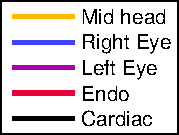
\includegraphics[]{../config/legend2.pdf} % TODO: vertical center
\hspace{0.3cm}
\begin{tabular}{c|cc|cc}
& \multicolumn{2}{c|}{Experiment} & \multicolumn{2}{c}{Control} \\
& Subject 1 & Subject 2 & Subject 1 & Subject 2 \\
\hline
\raisebox{-0.5\height}{\rotatebox{90}{VEP On}} &
\raisebox{-0.5\height}{\includegraphics[scale=0.32]{../vep/matlab_data/_Thu_15_05_2014_11_57_42_vep__labelled-crop.pdf}} &
\raisebox{-0.5\height}{\includegraphics[scale=0.32]{../vep/matlab_data/_Tue_06_05_2014_11_17_10_vep_-crop.pdf}} &
\raisebox{-0.5\height}{\includegraphics[scale=0.32]{../vep/matlab_data/_Thu_15_05_2014_12_15_47_vep_ctr-crop.pdf}} &
\raisebox{-0.5\height}{\includegraphics[scale=0.32]{../vep/matlab_data/_Tue_06_05_2014_11_25_22_vep_-crop.pdf}} \\
\raisebox{-0.5\height}{\rotatebox{90}{VEP Off}} &
\raisebox{-0.5\height}{\includegraphics[scale=0.32]{../vep/matlab_data/_Thu_15_05_2014_11_57_42_vep__off_labelled-crop.pdf}} &
\raisebox{-0.5\height}{\includegraphics[scale=0.32]{../vep/matlab_data/_Tue_06_05_2014_11_17_10_vep__off-crop.pdf}} &
\raisebox{-0.5\height}{\includegraphics[scale=0.32]{../vep/matlab_data/_Thu_15_05_2014_12_15_47_vep_ctr_off-crop.pdf}} &
\raisebox{-0.5\height}{\includegraphics[scale=0.32]{../vep/matlab_data/_Tue_06_05_2014_11_25_22_vep__off-crop.pdf}} \\
\raisebox{-0.5\height}{\rotatebox{90}{SSAEP 86 Hz}} &
\raisebox{-0.5\height}{\includegraphics[scale=0.32]{../ssavep/matlab_data/_Thu_15_05_2014_14_26_54_ssaep_86_labelled-crop.pdf}} &
\raisebox{-0.5\height}{\includegraphics[scale=0.32]{../ssavep/matlab_data/_Tue_06_05_2014_11_37_22_ssaep_86-crop.pdf}} &
\raisebox{-0.5\height}{\includegraphics[scale=0.32]{../ssavep/matlab_data/_Thu_15_05_2014_12_26_26_ssaep_ctr_86-crop.pdf}} &
\raisebox{-0.5\height}{\includegraphics[scale=0.32]{../ssavep/matlab_data/_Tue_06_05_2014_11_42_15_ssaep_86-crop.pdf}} \\
\raisebox{-0.5\height}{\rotatebox{90}{SSVEP 40 Hz}} &
\raisebox{-0.5\height}{\includegraphics[scale=0.32]{../ssavep/matlab_data/_Thu_15_05_2014_14_20_24_ssvep_40_labelled-crop.pdf}} &
\raisebox{-0.5\height}{\includegraphics[scale=0.32]{../ssavep/matlab_data/_Tue_06_05_2014_11_14_51_ssvep_40-crop.pdf}} &
\raisebox{-0.5\height}{\includegraphics[scale=0.32]{../ssavep/matlab_data/_Thu_15_05_2014_12_13_26_ssvep_ctr_40-crop.pdf}} &
\raisebox{-0.5\height}{\includegraphics[scale=0.32]{../ssavep/matlab_data/_Tue_06_05_2014_11_23_01_ssvep_40-crop.pdf}}
\end{tabular}
\caption{Performance of the electrodes at the optimal location for the endovascular location compared with the performance on the live control trials. The SSAEP and SSVEP experimental trials for Subject 1 are shown for the mid-basilar location. All other performances are shown at the basilar tip position. In each of the experiments, all experimental trials elicited a much larger response than the control experiments, which indicates that true non-artifactual responses were recorded. In addition, the endovascular electrode achieved superior signals compared to the scalp electrodes for the VEP and SSAEP experiments.}
% Figure 2
\end{center}
\end{figure}
\setlength{\tabcolsep}{6pt}

\setlength{\tabcolsep}{2pt}
\begin{figure}[H]
\begin{center}
\begin{tabular}{c|cccc|cc}
         & \multicolumn{4}{c|}{Experiment}                       & \multicolumn{2}{c}{Control} \\
         &             &             &             &             & Live         & Dead \\
\hline
Location & Basilar Tip & Mid-Basilar & VB Junction & Basilar Tip & Basilar Tip  & Basilar Tip \\
Time     & 11:57:42    & 14:13:26    & 15:54:54    & 16:47:47    & 12:15:47     & 17:22:22 \\
Time     & 0:00:00 & 2:15:44 & 3:57:12 & 4:50:05 & 0:18:05 & 5:24:40 \\ % TODO: time relative to anesthesia? relative to surgery
\hline
\raisebox{-0.5\height}{\rotatebox{90}{VEP On}} &
\raisebox{-0.5\height}{\includegraphics[scale=0.32]{../vep/matlab_data/_Thu_15_05_2014_11_57_42_vep__labelled-crop.pdf}} &
\raisebox{-0.5\height}{\includegraphics[scale=0.32]{../vep/matlab_data/_Thu_15_05_2014_14_13_26_vep_-crop.pdf}} &
\raisebox{-0.5\height}{\includegraphics[scale=0.32]{../vep/matlab_data/_Thu_15_05_2014_15_54_54_vep_-crop.pdf}} &
\raisebox{-0.5\height}{\includegraphics[scale=0.32]{../vep/matlab_data/_Thu_15_05_2014_16_47_47_vep_-crop.pdf}} &
\raisebox{-0.5\height}{\includegraphics[scale=0.32]{../vep/matlab_data/_Thu_15_05_2014_12_15_47_vep_ctr-crop.pdf}} &
\raisebox{-0.5\height}{\includegraphics[scale=0.32]{../vep/matlab_data/_Thu_15_05_2014_17_22_22_vep_-crop.pdf}} \\
\raisebox{-0.5\height}{\rotatebox{90}{VEP Off}} &
\raisebox{-0.5\height}{\includegraphics[scale=0.32]{../vep/matlab_data/_Thu_15_05_2014_11_57_42_vep__off_labelled-crop.pdf}} &
\raisebox{-0.5\height}{\includegraphics[scale=0.32]{../vep/matlab_data/_Thu_15_05_2014_14_13_26_vep__off-crop.pdf}} &
\raisebox{-0.5\height}{\includegraphics[scale=0.32]{../vep/matlab_data/_Thu_15_05_2014_15_54_54_vep__off-crop.pdf}} &
\raisebox{-0.5\height}{\includegraphics[scale=0.32]{../vep/matlab_data/_Thu_15_05_2014_16_47_47_vep__off-crop.pdf}} &
\raisebox{-0.5\height}{\includegraphics[scale=0.32]{../vep/matlab_data/_Thu_15_05_2014_12_15_47_vep_ctr_off-crop.pdf}} &
\raisebox{-0.5\height}{\includegraphics[scale=0.32]{../vep/matlab_data/_Thu_15_05_2014_17_22_22_vep__off-crop.pdf}} \\
\raisebox{-0.5\height}{\rotatebox{90}{SSAEP 86 Hz}} &
\raisebox{-0.5\height}{\includegraphics[scale=0.32]{../ssavep/matlab_data/_Thu_15_05_2014_12_31_02_ssaep_86_labelled-crop.pdf}} &
\raisebox{-0.5\height}{\includegraphics[scale=0.32]{../ssavep/matlab_data/_Thu_15_05_2014_14_26_54_ssaep_86-crop.pdf}} &
\raisebox{-0.5\height}{\includegraphics[scale=0.32]{../ssavep/matlab_data/_Thu_15_05_2014_16_12_19_ssaep_86-crop.pdf}} &
\raisebox{-0.5\height}{\includegraphics[scale=0.32]{../ssavep/matlab_data/_Thu_15_05_2014_16_58_34_ssaep_86-crop.pdf}} &
\raisebox{-0.5\height}{\includegraphics[scale=0.32]{../ssavep/matlab_data/_Thu_15_05_2014_12_26_26_ssaep_ctr_86-crop.pdf}} &
\raisebox{-0.5\height}{\includegraphics[scale=0.32]{../ssavep/matlab_data/_Thu_15_05_2014_17_12_38_ssaep_86-crop.pdf}} \\
\raisebox{-0.5\height}{\rotatebox{90}{SSVEP 40 Hz}} &
\raisebox{-0.5\height}{\includegraphics[scale=0.32]{../ssavep/matlab_data/_Thu_15_05_2014_12_08_22_ssvep_40_labelled-crop.pdf}} &
\raisebox{-0.5\height}{\includegraphics[scale=0.32]{../ssavep/matlab_data/_Thu_15_05_2014_14_20_24_ssvep_40-crop.pdf}} &
\raisebox{-0.5\height}{\includegraphics[scale=0.32]{../ssavep/matlab_data/_Thu_15_05_2014_16_02_44_ssvep_40-crop.pdf}} &
\raisebox{-0.5\height}{\includegraphics[scale=0.32]{../ssavep/matlab_data/_Thu_15_05_2014_16_38_47_ssvep_40-crop.pdf}} &
\raisebox{-0.5\height}{\includegraphics[scale=0.32]{../ssavep/matlab_data/_Thu_15_05_2014_12_13_26_ssvep_ctr_40-crop.pdf}} &
\raisebox{-0.5\height}{\includegraphics[scale=0.32]{../ssavep/matlab_data/_Thu_15_05_2014_17_18_01_ssvep_40-crop.pdf}}
\end{tabular}
\caption{Demonstration of position dependence for Subject 1. The performance of the endovascular electrode varies as its location is changed. The performance is consistent between the two basilar tip trials. }
% Figure 3
\end{center}
\end{figure}
\setlength{\tabcolsep}{6pt}

\begin{figure}[H]
\begin{center}
\begin{tabular}{cc}
\includegraphics[scale=0.5]{impedance.pdf}
\end{tabular}
\caption{Impedence characterization.} % Figure 4
\end{center}
\end{figure}

%\begin{figure}[H]
%\begin{center}
%\begin{tabular}{cc}
%\multirow{2}{*}{
%\begin{tabular}{ccc}
%Raw Trace & VEP Aligned & \\
%\raisebox{-0.5\height}{\includegraphics[scale=0.32]{../qrs/matlab_data/_Thu_15_05_2014_14_13_26_vep__start-crop.pdf}} &
%\raisebox{-0.5\height}{\includegraphics[scale=0.32]{../vep/matlab_data/_Thu_15_05_2014_14_13_26_vep__cardiac_labelled-crop.pdf}} &
%\\
%\raisebox{-0.5\height}{\includegraphics[scale=0.32]{../qrs/matlab_data/_Thu_15_05_2014_14_13_26_vep__end-crop.pdf}} &
%\raisebox{-0.5\height}{\includegraphics[scale=0.32]{../vep/matlab_data/_Thu_15_05_2014_14_13_26_vep__labelled-crop.pdf}} &
%\end{tabular}} &
%\raisebox{-0.5\height}{cardiac aligned avg vep + EKG} \\
%& \raisebox{-0.5\height}{\includegraphics[scale=0.32]{../qrs/matlab_data/_Thu_15_05_2014_14_13_26_vep__qrs-crop.pdf}} \\
%%\raisebox{-0.5\height}{contaminated raw trace + cardiac} &
%%\raisebox{-0.5\height}{VEP aligned contaminated EKG} &
%%\raisebox{-0.5\height}{vep aligned cleaned} &
%%\raisebox{-0.5\height}{raw cleaned} &
%%\raisebox{-0.5\height}{\includegraphics[scale=0.32]{../qrs/matlab_data/_Thu_15_05_2014_14_13_26_vep__end-crop.pdf}}
%\end{tabular}

%\begin{figure}[H]
%\begin{center}
%\begin{tabular}{cccc}
%& Raw Trace & VEP Aligned & cardiac aligned avg vep + EKG \\
%\raisebox{-0.5\height}{\rotatebox{90}{Contaminated}} &
%\raisebox{-0.5\height}{\includegraphics[scale=0.32]{../qrs/matlab_data/_Thu_15_05_2014_14_13_26_vep__start-crop.pdf}} &
%\raisebox{-0.5\height}{\includegraphics[scale=0.32]{../vep/matlab_data/_Thu_15_05_2014_14_13_26_vep__cardiac_labelled-crop.pdf}} &
%\raisebox{-0.5\height}{\multirow{2}{*}{\includegraphics[scale=0.64]{../qrs/matlab_data/_Thu_15_05_2014_14_13_26_vep__qrs-crop.pdf}}} \\
%\raisebox{-0.5\height}{\rotatebox{90}{Cleaned}} &
%\raisebox{-0.5\height}{\includegraphics[scale=0.32]{../qrs/matlab_data/_Thu_15_05_2014_14_13_26_vep__end-crop.pdf}} &
%\raisebox{-0.5\height}{\includegraphics[scale=0.32]{../vep/matlab_data/_Thu_15_05_2014_14_13_26_vep__labelled-crop.pdf}} &
%\end{tabular}

\begin{figure}[H]
\begin{center}
\begin{tabular}{cc|cc}
\raisebox{-0.5\height}{\multirow{3}{*}{
\begin{tabular}{c}
Cardiac-Aligned  Measurements \vspace{0.7cm} \\
\includegraphics[scale=0.64]{../qrs/matlab_data/_Thu_15_05_2014_14_13_26_vep__qrs-crop.pdf}
\end{tabular}
}} &
& Raw Trace & VEP-Aligned \\
\hline
&
\raisebox{-0.5\height}{\rotatebox{90}{Contaminated}} &
\raisebox{-0.5\height}{\includegraphics[scale=0.32]{../qrs/matlab_data/_Thu_15_05_2014_14_13_26_vep__start-crop.pdf}} &
\raisebox{-0.5\height}{\includegraphics[scale=0.32]{../vep/matlab_data/_Thu_15_05_2014_14_13_26_vep__cardiac_labelled-crop.pdf}} \\
&
\raisebox{-0.5\height}{\rotatebox{90}{Cleaned}} &
\raisebox{-0.5\height}{\includegraphics[scale=0.32]{../qrs/matlab_data/_Thu_15_05_2014_14_13_26_vep__end-crop.pdf}} &
\raisebox{-0.5\height}{\includegraphics[scale=0.32]{../vep/matlab_data/_Thu_15_05_2014_14_13_26_vep__labelled-crop.pdf}} \\
\end{tabular}


\caption{Cardiac contamination and cleaning. 1076 trials for qrs mean} % Figure 5
\end{center}
\end{figure}


%% VEP 
%filename: _Tue_06.05.2014_11%3A17%3A10_vep_,    2 / 13
%Number of Trials: 153
%Number of Trials: 153
%filename: _Thu_15.05.2014_11%3A57%3A42_vep_,    4 / 16
%Number of Trials: 205
%Number of Trials: 206
%filename: _Thu_15.05.2014_14%3A13%3A26_vep_,    10 / 16
%Number of Trials: 192
%Number of Trials: 191
%filename: _Thu_15.05.2014_15%3A54%3A54_vep_,    12 / 16
%Number of Trials: 208
%Number of Trials: 208
%filename: _Thu_15.05.2014_16%3A47%3A47_vep_,    15 / 16
%Number of Trials: 208
%Number of Trials: 208
%filename: _Thu_15.05.2014_12%3A15%3A47_vep_ctr, 5 / 16
%Number of Trials: 208
%Number of Trials: 208
%filename: _Thu_15.05.2014_17%3A22%3A22_vep_,    16 / 16
%Number of Trials: 208
%Number of Trials: 208
%filename: _Tue_06.05.2014_11%3A25%3A22_vep_,    3 / 13
%Number of Trials: 153
%Number of Trials: 153
%filename: _Thu_15.05.2014_14%3A13%3A26_vep_,    10 / 16
%Number of Trials: 192
%Number of Trials: 191


%% SSAVEP
%filename: _Thu_15.05.2014_12%3A08%3A22_ssvep_40,    11 / 39
%Experiment: 320640 584434
%Baseline: 9600 301440
%filename: _Thu_15.05.2014_12%3A31%3A02_ssaep_86,    15 / 40
%Experiment: 307603 585728
%Baseline: 9600 288403
%filename: _Tue_06.05.2014_11%3A14%3A51_ssvep_40,    5 / 39
%Experiment: 320045 583839
%Baseline: 9600 300845
%filename: _Tue_06.05.2014_11%3A37%3A22_ssaep_86,    8 / 41
%Experiment: 70740 585728
%Baseline: 9600 51540
%filename: _Tue_06.05.2014_11%3A23%3A01_ssvep_40,    8 / 39
%Experiment: 317488 581282
%Baseline: 9600 298288
%filename: _Tue_06.05.2014_11%3A42%3A15_ssaep_86,    11 / 41
%Experiment: 94848 585856
%Baseline: 9600 75648
%filename: _Thu_15.05.2014_12%3A13%3A26_ssvep_ctr_40,    14 / 39
%Experiment: 328552 592346
%Baseline: 9600 309352
%filename: _Thu_15.05.2014_12%3A26%3A26_ssaep_ctr_86,    12 / 40
%Experiment: 305364 585856
%Baseline: 9600 286164
%filename: _Thu_15.05.2014_09%3A52%3A53_ssvep_40,    2 / 39
%Experiment: 328875 592669
%Baseline: 9600 309675
%filename: _Thu_15.05.2014_12%3A08%3A22_ssvep_40,    11 / 39
%Experiment: 320640 584434
%Baseline: 9600 301440
%filename: _Thu_15.05.2014_14%3A20%3A24_ssvep_40,    23 / 39
%Experiment: 323398 587192
%Experiment: 371398 587192
%Baseline: 9600 304198
%filename: _Thu_15.05.2014_16%3A02%3A44_ssvep_40,    32 / 39
%Experiment: 609145 1156050
%Baseline: 9600 589945
%filename: _Thu_15.05.2014_16%3A38%3A47_ssvep_40,    35 / 39
%Experiment: 611121 1158026
%Baseline: 9600 591921
%filename: _Thu_15.05.2014_12%3A13%3A26_ssvep_ctr_40,    14 / 39
%Experiment: 328552 592346
%Baseline: 9600 309352
%filename: _Thu_15.05.2014_17%3A18%3A01_ssvep_40,    38 / 39
%Experiment: 606919 1153824
%Baseline: 9600 587719
%filename: _Thu_15.05.2014_10%3A04%3A16_ssaep_86,    3 / 40
%Experiment: 303843 585856
%Baseline: 9600 284643
%filename: _Thu_15.05.2014_12%3A31%3A02_ssaep_86,    15 / 40
%Experiment: 307603 585728
%Baseline: 9600 288403
%filename: _Thu_15.05.2014_14%3A26%3A54_ssaep_86,    24 / 40
%Experiment: 301020 585728
%Baseline: 9600 281820
%filename: _Thu_15.05.2014_16%3A12%3A19_ssaep_86,    33 / 40
%Experiment: 593190 1161856
%Baseline: 9600 573990
%filename: _Thu_15.05.2014_16%3A58%3A34_ssaep_86,    36 / 40
%Experiment: 595230 1161728
%Baseline: 9600 576030
%filename: _Thu_15.05.2014_12%3A26%3A26_ssaep_ctr_86,    12 / 40
%Experiment: 305364 585856
%Baseline: 9600 286164
%filename: _Thu_15.05.2014_17%3A12%3A38_ssaep_86,    40 / 40
%Experiment: 595109 1161728
%Baseline: 9600 575909

\end{document}

